\chapter{Gaussian Process}
  \lettrine[lines=2]{G}aussian Process (sometimes abbreviated as GP) is a supervised learning model that found large application
  in the domain of regression, classification and clustering. In this appendix we focus on application
  of GPs over a generic regression problem.\newline
  There are many ways to interpret this type of model, for this section we will focus on the \textit{weight-space view} and
  on the \textit{function-space view}. The latter interpret a gaussian process as an entity defining a distribution over
  function, hence the name, and inference taking place directly inside the space of the functions. On the other hand the
  weight-space view is simpler to grasp  but at the same time completely equivalent with the first interpretation.\newline

  \noindent The appendix is divided into two main section, representing the two way to interpret a GP model. The main results
  known in literature are given. It also important to remark that this appendix is of fundamental importance in our work
  given that the entire weight estimation procedure for WFQI relies on gaussian processes.

  \section{Weight-Space View}
    \noindent We start our discussion with the weight-space view given that it can be obtained starting from a
    simple linear regression model.
    \subsection{Bayesian Linear Regression}
      \noindent We initially consider the usual linear regression model
      \begin{equation*}
        f(\pmb{x}) = \pmb{x}^{t} \pmb{w} \quad \quad y = f(\pmb{x}) + \epsilon
      \end{equation*}
      where $\pmb{x} \in \mathbb{R}^n$ is the input variable, $f$ is true function we are trying to fit,
      $\pmb{w}$ is the vector of the weight and $y \in \mathbb{R}$ is the observed target value.\newline
      $\epsilon$ is the additive \textbf{gaussian} noise we suppose is present in the observed samples. In particular we have
      \begin{equation*}
        \epsilon \sim \mathcal{N}(0,\sigma^{2}_{e})
      \end{equation*}
      Under independence assumption of the observation, we can write the likelihood function of our model (ie. the probability that
      our model has generated the observed target):
      \begin{equation}
        \label{likelihood}
        p(\pmb{y}|\pmb{X},\pmb{w}) = \prod_{i=1}^{n} p(y_{i}|\pmb{x}_{i},\pmb{w}) = \prod_{i=1}^{n} \frac{1}{\sqrt{2\pi}\sigma_{e}} e^{-\frac{(y_{i}-\pmb{x}_{i}^{t} \pmb{w})^{2}} {2\sigma^{2}_{e}}} =
        \mathcal{N}(\pmb{X}^{t}\pmb{w}, \sigma^{2}_{e} \pmb{I})
      \end{equation}
      where $\pmb{I}$ indicates the identity matrix of order $n$.\newline

      \noindent As in every bayesian setting we need to specify a prior distribution over the space of the variables we are going
      to fit, in our case we need to specify a probability distribution over $\pmb{w}$ and for this discussion we assume:
      \begin{equation*}
        \pmb{w} \sim \mathcal{N}(\pmb{0}, \Sigma_p)
      \end{equation*}

      \noindent To make inference possible in this context we need the posterior distribution, that, given the prior over the parameters
      can be easily obtained using the Bayes theorem:
      \begin{equation}
        p(\pmb{w}|\pmb{y},\pmb{X}) = \frac{p(\pmb{y}|\pmb{X},\pmb{w}) p(\pmb{w})}{p(\pmb{y}|\pmb{X})}
      \end{equation}
      Note that $p(\pmb{y}|\pmb{X})$, known as marginal distribution, is independent from $\pmb{w}$ and acts only as
      a normalizing factor.\newline

      \noindent With some simple algebraic manipulation we obtain the following result for the posterior distribution:
      \begin{equation}
        \begin{split}
          p(\pmb{w}|\pmb{X},\pmb{y}) = \mathcal{N}(\bar{\pmb{w}}, A^{-1}) \\
          \bar{\pmb{w}} = \frac{1}{\sigma^{2}_{e}} A^{-1} \pmb{X} \pmb{y} \\
          A = \frac{\pmb{X}\pmb{X}^t}{\sigma^{2}_e} + \Sigma_{p}^{-1}
        \end{split}
        \label{posterior}
      \end{equation}

      \noindent Given that in gaussian settings the mode coincide with the mean of the distribution this is, by construction a
      Maximum a Posteriori (MAP) estimator.\newline

      \noindent Finally we want to make predictions: this is possible by averaging all the possible parameters value \textit{weighted}
      by their posterior probability. With other words the prediction for a new test input is given by averaging
      the output of all the possible linear model with respect to the gaussian posterior distribution. In formula:
      \begin{equation*}
        p(\pmb{y}^{*}|\pmb{x}^{*}, \pmb{X}, \pmb{y}) = \int p(\pmb{y}^{*}|\pmb{x}^{*}, \pmb{w}) p(\pmb{w}|\pmb{X},\pmb{y}) d\pmb{w} = \mathcal{N}(\frac{1}{\sigma^{2}_{e}} \pmb{x}_{*}^{t} A^{-1} \pmb{X} \pmb{y}, \pmb{x}_{*}^{t} A^{-1} \pmb{x}_{*})
      \end{equation*}

      \noindent It is important to notice that the predictive distribution is gaussian with a mean given by the posterior mean of
      the weights from eq. \ref{posterior} multiplied by the test input.\newline

      \noindent The model obtain is a simple version of a linear gaussian process. In the next section we describe an extended version
      of the previous model by projecting the input space in the feature space.

    \subsection{Kernel Trick}
      \noindent In the previous paragraph we have described a simple linear model which suffers from very limited expressiveness.
      To expand the previous model we introduce a new function $\phi$ that maps the $n$-dimensional vector $\pmb{x}$ to
      an $N$-dimensional feature space.\newline
      Our model is now
      \begin{equation}
        f(\pmb{x}) = \phi(\pmb{x})^t \pmb{w}
      \end{equation}

      \noindent All the equations stated in the previous section do not change except by substituting $\pmb{X}$ with $\Phi(\pmb{X})$ where
      the latter expression is an abbreviated formula to indicate the columns $\phi(\pmb{x})$ for all the possible choices of $\pmb{x}$.\newline

      \noindent A computationally efficient expression for the predictive distribution that takes in account the projection is given by the following equation:
      \begin{equation}
        p(\pmb{y}^{*}|\pmb{x}^{*}, \pmb{X}, \pmb{y}) = \mathcal{N}(\phi_{*}^{T} \Sigma_{p} \Phi (K + \sigma_{p}^{2} \pmb{I})^{-1} \pmb{y}, \phi_{*}^{T} \Sigma_{p} \phi_{*} - \phi_{*}^{T} \Sigma_{p} \Phi(K + \sigma_{p}^{2} \pmb{I})^{-1} \phi_{*}^{T} \Sigma_{p} \phi_{*})
      \end{equation}
      where $K = \Phi^{T} \Sigma_{p} \Phi$.\newline
      \noindent It is know important to notice the the recurrence of the term $\phi(\pmb{x}) \Sigma_{p} \phi(\pmb{x})$. We define $\psi(\pmb{x}) = \Sigma_{p}^{1/2} \phi(\pmb{x})$.
      The \textit{kernel trick} consists in defining $k(\pmb{x},\pmb{x}') = \psi(\pmb{x}) \psi(\pmb{x}')$. $k$ is known as \textit{covariance function} or simply as \textit{kernel function}.
      This substitution permit to use an arbitrary kernel function and does not require to compute the product between the features vectors which in general
      results to be computationally expensive.

  \section{Function-Space View}
    \noindent The function-space view represents an equivalent way to look at Gaussian Process. First we give a formal definition

    \begin{definition}
      A Gaussian process is a collection of random variables, any finite number of which have a joint Gaussian distribution.
    \end{definition}

    \noindent In this setting a GP is completely specified by a \textit{mean and covariance function}. Let $f(\pmb{x})$ be a GP than
    \begin{equation}
      \begin{cases}
        m(\pmb{x}) = \mathbb{E}[f(\pmb{x})] \\
        k(\pmb{x},\pmb{x}') = \mathbb{E}[(f(\pmb{x}) - m(\pmb{x})) (f(\pmb{x}') - m(\pmb{x}'))]
      \end{cases}
    \end{equation}

    \noindent It is important to notice that this definition is completely in accordance with the weight-space view. Indeed our
    simple linear bayesian regression model can be obtained by defining:
    \begin{equation}
      \begin{cases}
        m(\pmb{x}) = \mathbb{E}[f(\pmb{x})] = \phi(\pmb{x})^{T} \mathbb{E}[\pmb{w}] = 0 \\
        k(\pmb{x},\pmb{x}') = \phi(\pmb{x})^{T} \Sigma_{p} \phi(\pmb{x}')
      \end{cases}
    \end{equation}

    \noindent The covariance function represents implies a distribution over the space of functions. Figure \ref{function_samples}
    shows, for different choice of the kernel function, samples of function drawn from the prior distribution. Again the choice
    of the covariance function is not arbitrary and requires some educated guesses and domain specific knowledge.\newline

    \noindent Prediction, in case of noise-free observations, for new test input happens in a symmetrical way with respect the bayesian model
    \begin{equation}
      \begin{multlined}
        \pmb{f}_{*} | \pmb{X}, \pmb{X}_{*}, \pmb{f} \sim \mathcal{N}(K(\pmb{X}_{*},\pmb{X})K(\pmb{X},\pmb{X})^{-1}\pmb{f}, \\ K(\pmb{X}_{*},\pmb{X}_{*}) - K(\pmb{X}_{*},\pmb{X}) K(\pmb{X},\pmb{X})^{-1}K(\pmb{X}_{*},\pmb{X}_{*}))
      \end{multlined}
    \end{equation}
    \begin{figure}
      \centering
      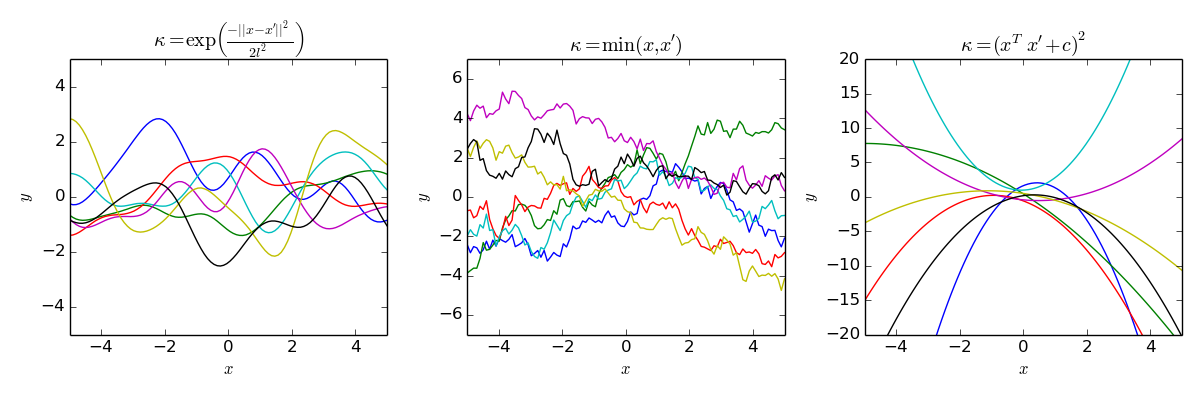
\includegraphics[scale=0.45]{images/covGP.png}
      \caption{Prior samples with different kernels}
      \label{function_samples}
    \end{figure}

    \noindent The previous equation can be extended also for the case of noisy observation by taking into account also the
    variance of the error ($\sigma^{2}_{e}$) associated with the observed data. 
